\documentclass[tikz,border=8pt]{standalone}
\usepackage[T1]{fontenc}
\usetikzlibrary{arrows.meta,backgrounds}
\definecolor{ink}{HTML}{24343C}
\definecolor{teal}{HTML}{247B79}
\definecolor{coral}{HTML}{AE5B47}

% Edge plan: source -> target | meaning | corridor.
% parser -> session | command syntax | top row, left to right.
% session -> frontend | translate active context | top row, left to right.
% frontend -> roots | construct typed assertions | right vertical band.
% roots -> ground | no quantified assertions | middle band, then down left.
% roots -> quantified | quantified UF assertions | right vertical band.
% ground -> outcome | finalized ground outcome | lower left, then inward.
% quantified -> outcome | quantified outcome | lower right, then inward.
% This is data flow in rebuild mode, not an ownership or call-stack diagram.
% Early errors, unsupported inputs, and preprocessing exits are not expanded.

\begin{document}
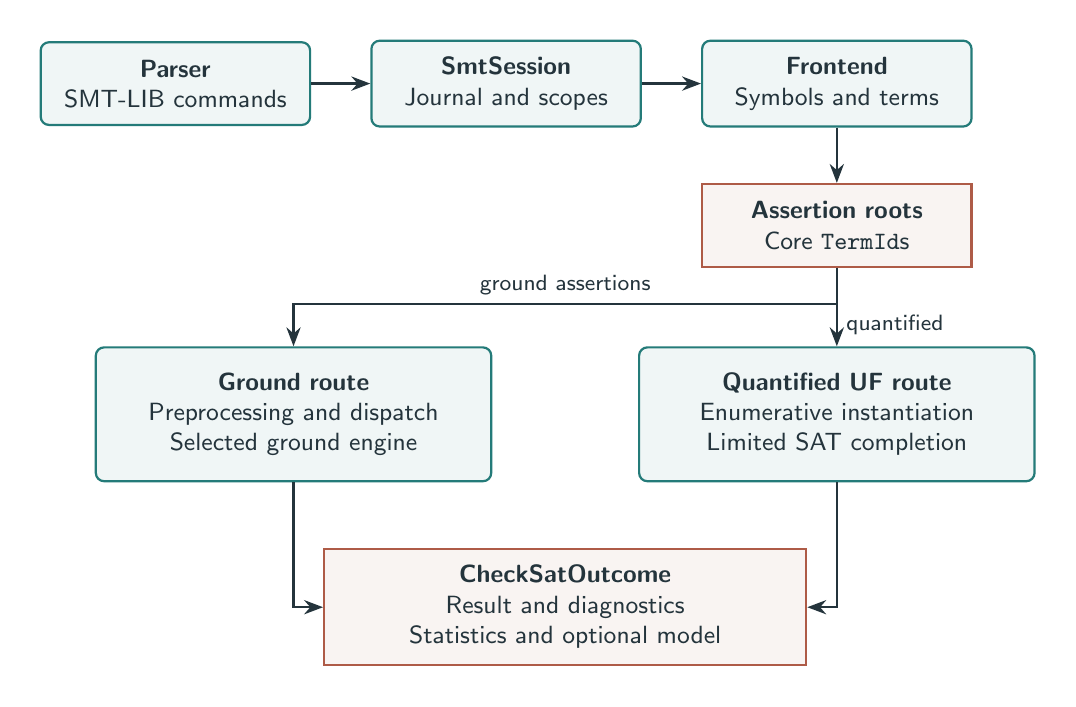
\begin{tikzpicture}[
  font=\sffamily\small, text=ink,
  every node/.style={align=center, inner sep=6pt},
  process/.style={draw=teal, fill=teal!7, rounded corners=3pt,
    text width=3.0cm, minimum height=1.05cm, line width=0.8pt},
  artifact/.style={draw=coral, fill=coral!7,
    text width=3.0cm, minimum height=1.05cm, line width=0.8pt},
  route/.style={process, text width=4.6cm, minimum height=1.7cm},
  flow/.style={-{Stealth[length=2.4mm]}, draw=ink, line width=0.9pt},
  label/.style={font=\sffamily\footnotesize, inner sep=3pt},
  background rectangle/.style={fill=white}, show background rectangle
]
  \node[process] (parser) at (0,0)
    {\textbf{Parser}\\SMT-LIB commands};
  \node[process] (session) at (4.2,0)
    {\textbf{SmtSession}\\Journal and scopes};
  \node[process] (frontend) at (8.4,0)
    {\textbf{Frontend}\\Symbols and terms};
  \node[artifact] (roots) at (8.4,-1.8)
    {\textbf{Assertion roots}\\Core \texttt{TermId}s};
  \node[route] (ground) at (1.5,-4.2)
    {\textbf{Ground route}\\Preprocessing and dispatch\\Selected ground engine};
  \node[route] (quantified) at (8.4,-4.2)
    {\textbf{Quantified UF route}\\Enumerative instantiation\\Limited SAT completion};
  \node[artifact, text width=5.7cm, minimum height=1.15cm] (outcome) at (4.95,-6.65)
    {\textbf{CheckSatOutcome}\\Result and diagnostics\\Statistics and optional model};

  \draw[flow] (parser.east) -- (session.west);
  \draw[flow] (session.east) -- (frontend.west);
  \draw[flow] (frontend.south) -- (roots.north);
  \coordinate (branch) at (8.4,-2.8);
  \draw[draw=ink, line width=0.9pt] (roots.south) -- (branch);
  \draw[flow] (branch) -- node[label, above] {ground assertions}
    (1.5,-2.8) -- (ground.north);
  \draw[flow] (branch) -- node[label, right] {quantified} (quantified.north);
  \draw[flow] (ground.south) -- (1.5,-6.65) -- (outcome.west);
  \draw[flow] (quantified.south) -- (8.4,-6.65) -- (outcome.east);
\end{tikzpicture}
\end{document}
